\subsection{Referencia}

La empresa requirió que se utilizara un brazo robótico en 3D diseñado por la propia empresa, e incluido en el software SettDev, para ser empleado como referencia del movimiento realizado por la ortesis. La Figura \ref{fig:referencia} muestra el brazo en 3D diseñado por la propia empresa. Puede notarse que en la parte superior hay controles deslizantes. La empresa requirió que estos controles mostraran los ángulos utilizados como referencia, es decir, que los ángulos aplicados para controlar el movimiento del brazo en 3D, se mostraran numéricamente en los controles deslizantes.

\begin{figure}[htb]
	\centering
	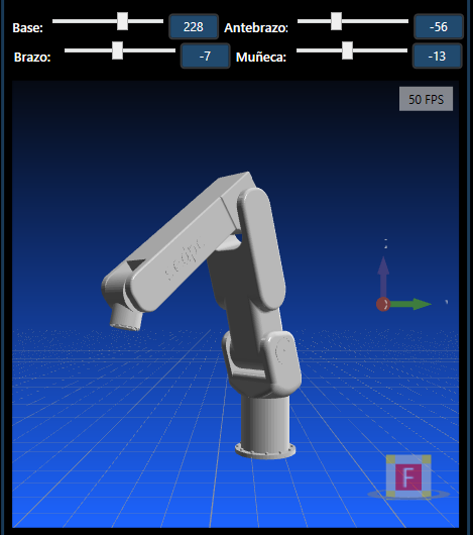
\includegraphics[scale=0.8]{referencia.png}
	\caption{Brazo en 3D utilizado como referencia en el software SettDev}
	\label{fig:referencia}
\end{figure}